\chapterfont{\centering}
\chapter[Chapter One Tittle: Some Formating Examples]{Chapter One Tittle:\\ Some Formating\\ Examples}\label{ch_one}
\section{Chapter one tittle section}
\subsection{Formating very, very, very long chapter titles}
The title of \Cref{ch_one} is an example how to deal with the chapter titles that do not fit in one line. Chapter titles should be in the shape of an inverted pyramid if more than one line of text. If only one line, center on the page. Use this trick for long chapter titles.

\subsection{Subsection of section - double quotes}
Example of double quotes ``word''. Lorem ipsum dolor sit amet, consectetur adipiscing elit. Curabitur viverra, velit eget vestibulum viverra, nisl eros aliquet sapien, sed interdum tellus justo et purus. Nulla vel orci nisl. Curabitur porta lacinia quam, finibus bibendum mi tincidunt eget. Aenean aliquam lobortis orci, ut aliquam neque imperdiet vel. Nunc sit amet scelerisque velit. Aenean quis tempor leo, at consectetur ipsum. Nam ac urna dapibus, condimentum orci a, ornare ante. In hac habitasse platea dictumst. 
\subsection{Another subsection of section - citations}
Example of citation \citep{altschul1997gapped}. Mauris nisi felis, pharetra vitae velit at, sollicitudin molestie justo. Aenean tristique diam pulvinar, semper risus sed, mattis elit. Phasellus interdum erat at enim maximus interdum. Curabitur tempor, arcu nec malesuada facilisis, tortor nisi ornare ex, ut porttitor elit lectus aliquam diam. Cum sociis natoque penatibus et magnis dis parturient montes, nascetur ridiculus mus. Vivamus quam turpis, auctor in nunc nec, varius pharetra nibh. Ut sagittis diam nec dui sodales tempor. Integer molestie diam id quam placerat eleifend. Nulla posuere iaculis nisi, et sagittis ipsum consequat scelerisque. In nec turpis eget tellus pulvinar porttitor vitae ac tortor. Nullam tempor ut orci ac porttitor. Pellentesque aliquam lacinia gravida. Duis accumsan tristique augue, vitae aliquam magna convallis ac. Aenean vel diam non eros venenatis ullamcorper sit amet at augue. 

Example of multiple citations \citep{altschul1997gapped,baker2007novel}. Nullam mollis et leo at pharetra. Nulla efficitur molestie euismod. Sed dapibus metus sed tempus varius. Aenean finibus eros ut urna luctus feugiat. Duis turpis risus, viverra vitae porta et, ullamcorper ac est. Proin in eros nec ipsum interdum tempus. Nam fringilla lectus velit, non posuere ex vehicula ut. Mauris tincidunt, dolor sit amet commodo tempor, erat mi egestas dui, at elementum tellus est rhoncus libero. Ut et rutrum lectus, id viverra tortor. Vivamus nec lacus eros. Donec dictum porta nisi et vestibulum. Mauris luctus ligula ut libero aliquet luctus. Quisque malesuada egestas finibus. 
\subsubsection{Subsubsection of section - italic text}
Example of italic text - {\it Escherichia}, {\it Salmonella}, and {\it Shigella} spp. Mauris dictum pharetra fermentum. Maecenas ut felis varius, dapibus sapien imperdiet, dictum dui. Proin feugiat viverra metus non laoreet. Integer pulvinar mi id lacus semper commodo. Praesent vel erat interdum purus scelerisque maximus. Sed enim risus, mollis blandit ligula ac, sagittis venenatis augue. Mauris nisi purus, gravida ac aliquam eu, ullamcorper eget nulla. Proin id finibus purus. Vestibulum leo ante, porta in quam sed, eleifend feugiat arcu. Nunc viverra fringilla turpis a iaculis. In condimentum aliquet mauris, quis laoreet eros porta eu. Aenean ut turpis a massa gravida pretium. Phasellus auctor purus quis diam interdum, nec luctus lorem auctor. Pellentesque finibus elit justo, a vulputate diam fermentum lacinia. 
\section{Another section}
Mauris dictum pharetra fermentum. Maecenas ut felis varius, dapibus sapien imperdiet, dictum dui. Proin feugiat viverra metus non laoreet. Integer pulvinar mi id lacus semper commodo. Praesent vel erat interdum purus scelerisque maximus. Sed enim risus, mollis blandit ligula ac, sagittis venenatis augue. Mauris nisi purus, gravida ac aliquam eu, ullamcorper eget nulla. Proin id finibus purus. Vestibulum leo ante, porta in quam sed, eleifend feugiat arcu. Nunc viverra fringilla turpis a iaculis. In condimentum aliquet mauris, quis laoreet eros porta eu. Aenean ut turpis a massa gravida pretium. Phasellus auctor purus quis diam interdum, nec luctus lorem auctor. Pellentesque finibus elit justo, a vulputate diam fermentum lacinia. 
\section{Another section}
Mauris dictum pharetra fermentum. Maecenas ut felis varius, dapibus sapien imperdiet, dictum dui. Proin feugiat viverra metus non laoreet. Integer pulvinar mi id lacus semper commodo. Praesent vel erat interdum purus scelerisque maximus. Sed enim risus, mollis blandit ligula ac, sagittis venenatis augue. Mauris nisi purus, gravida ac aliquam eu, ullamcorper eget nulla. Proin id finibus purus. Vestibulum leo ante, porta in quam sed, eleifend feugiat arcu. Nunc viverra fringilla turpis a iaculis. In condimentum aliquet mauris, quis laoreet eros porta eu. Aenean ut turpis a massa gravida pretium. Phasellus auctor purus quis diam interdum, nec luctus lorem auctor. Pellentesque finibus elit justo, a vulputate diam fermentum lacinia. 

\chapter{Chapter Two Tittle: Links}
\section{Chapter one tittle section - links examples}
Example of hyperlink \url{http://www.wikibooks.org}. Fusce ultricies pulvinar diam sed ultrices. Sed orci justo, rutrum in dolor a, consequat dictum mi. Sed luctus congue ex nec dignissim. Phasellus volutpat urna vestibulum ipsum vestibulum, quis venenatis justo consectetur. Nullam hendrerit nisl in rutrum convallis. Sed sit amet malesuada nisi. Phasellus dolor neque, vehicula vestibulum semper at, facilisis eget libero. Mauris interdum magna molestie, auctor felis a, condimentum odio. Pellentesque habitant morbi tristique senectus et netus et malesuada fames ac turpis egestas. Suspendisse maximus lacinia dignissim. Maecenas pharetra accumsan metus, sagittis dictum purus sollicitudin eget. Curabitur ut porttitor arcu, ut porttitor ipsum. Vestibulum porttitor finibus sapien, ac pharetra odio bibendum nec. Nullam tincidunt dignissim risus imperdiet dictum.

Pellentesque habitant morbi tristique senectus et netus et malesuada fames ac turpis egestas. Suspendisse maximus lacinia dignissim. Maecenas pharetra accumsan metus, sagittis dictum purus sollicitudin eget. Curabitur ut porttitor arcu, ut porttitor ipsum. Vestibulum porttitor finibus sapien, ac pharetra odio bibendum nec. Nullam tincidunt dignissim risus imperdiet dictum.
\subsection{Subsection title - more links examples}.
Another example of hyperlink \href{http://www.wikibooks.org}{Wikibooks home}. Nullam mollis et leo at pharetra. Nulla efficitur molestie euismod. Sed dapibus metus sed tempus varius. Aenean finibus eros ut urna luctus feugiat. Duis turpis risus, viverra vitae porta et, ullamcorper ac est. Proin in eros nec ipsum interdum tempus. Nam fringilla lectus velit, non posuere ex vehicula ut. Mauris tincidunt, dolor sit amet commodo tempor, erat mi egestas dui, at elementum tellus est rhoncus libero. Ut et rutrum lectus, id viverra tortor. Vivamus nec lacus eros. Donec dictum porta nisi et vestibulum. Mauris luctus ligula ut libero aliquet luctus. Quisque malesuada egestas finibus.

\section{Another Section}
\subsection{Subsection title}.
Pellentesque habitant morbi tristique senectus et netus et malesuada fames ac turpis egestas. Suspendisse maximus lacinia dignissim. Maecenas pharetra accumsan metus, sagittis dictum purus sollicitudin eget. Curabitur ut porttitor arcu, ut porttitor ipsum. Vestibulum porttitor finibus sapien, ac pharetra odio bibendum nec. Nullam tincidunt dignissim risus imperdiet dictum.

\chapter[Chapter Three Title: Mathematics Notations]{Chapter Three Title:\\ Mathematics\\ Notations}
\section{Some Math Stuff}
LaTeX{} has a special way to embed mathematical symbols and notations. Here are some of them. Also observe how a bullet list is made.
\begin{itemize}\itemsep0pt \parskip0pt \parsep0pt
\item greater than $\ge$
\item less than $\le$
\item percent sign \%
\item multiply $N\times N$
\item inline equation $M = N(N-1)/2$
\end{itemize}
Sed orci justo, rutrum in dolor a, consequat dictum mi. Sed luctus congue ex nec dignissim. Phasellus volutpat urna vestibulum ipsum vestibulum, quis venenatis justo consectetur. Nullam hendrerit nisl in rutrum convallis. Sed sit amet malesuada nisi. Phasellus dolor neque, vehicula vestibulum semper at, facilisis eget libero. Mauris interdum magna molestie, auctor felis a, condimentum odio. Pellentesque habitant morbi tristique senectus et netus et malesuada fames ac turpis egestas. Suspendisse maximus lacinia dignissim. Maecenas pharetra accumsan metus, sagittis dictum purus sollicitudin eget. Curabitur ut porttitor arcu, ut porttitor ipsum. Vestibulum porttitor finibus sapien, ac pharetra odio bibendum nec. Nullam tincidunt dignissim risus imperdiet dictum.

Pellentesque habitant morbi tristique senectus et netus et malesuada fames ac turpis egestas. Suspendisse maximus lacinia dignissim. Maecenas pharetra accumsan metus, sagittis dictum purus sollicitudin eget. Curabitur ut porttitor arcu, ut porttitor ipsum. Vestibulum porttitor finibus sapien, ac pharetra odio bibendum nec. Nullam tincidunt dignissim risus imperdiet dictum.
\section{Math equation}
Example of a mathematical formula:
\begin{equation}
  ADD = \sum_{i=1}^{M}|<D(n+1,i)>-<D(n,i)>|
  \label{add}
\end{equation}

Pellentesque habitant morbi tristique senectus et netus et malesuada fames ac turpis egestas. Suspendisse maximus lacinia dignissim. Maecenas pharetra accumsan metus, sagittis dictum purus sollicitudin eget. Curabitur ut porttitor arcu, ut porttitor ipsum. Vestibulum porttitor finibus sapien, ac pharetra odio bibendum nec. Nullam tincidunt dignissim risus imperdiet dictum.
\section{Chapter section}
Fusce ultricies pulvinar diam sed ultrices. Sed orci justo, rutrum in dolor a, consequat dictum mi. Sed luctus congue ex nec dignissim. Phasellus volutpat urna vestibulum ipsum vestibulum, quis venenatis justo consectetur. Nullam hendrerit nisl in rutrum convallis. Sed sit amet malesuada nisi. Phasellus dolor neque, vehicula vestibulum semper at, facilisis eget libero. Mauris interdum magna molestie, auctor felis a, condimentum odio. Pellentesque habitant morbi tristique senectus et netus et malesuada fames ac turpis egestas. Suspendisse maximus lacinia dignissim. Maecenas pharetra accumsan metus, sagittis dictum purus sollicitudin eget. Curabitur ut porttitor arcu, ut porttitor ipsum. Vestibulum porttitor finibus sapien, ac pharetra odio bibendum nec. Nullam tincidunt dignissim risus imperdiet dictum.

Pellentesque habitant morbi tristique senectus et netus et malesuada fames ac turpis egestas. Suspendisse maximus lacinia dignissim. Maecenas pharetra accumsan metus, sagittis dictum purus sollicitudin eget. Curabitur ut porttitor arcu, ut porttitor ipsum. Vestibulum porttitor finibus sapien, ac pharetra odio bibendum nec. Nullam tincidunt dignissim risus imperdiet dictum.

\section{Chapter section}
Fusce ultricies pulvinar diam sed ultrices. Sed orci justo, rutrum in dolor a, consequat dictum mi. Sed luctus congue ex nec dignissim. Phasellus volutpat urna vestibulum ipsum vestibulum, quis venenatis justo consectetur. Nullam hendrerit nisl in rutrum convallis. Sed sit amet malesuada nisi. Phasellus dolor neque, vehicula vestibulum semper at, facilisis eget libero. Mauris interdum magna molestie, auctor felis a, condimentum odio. Pellentesque habitant morbi tristique senectus et netus et malesuada fames ac turpis egestas. Suspendisse maximus lacinia dignissim. Maecenas pharetra accumsan metus, sagittis dictum purus sollicitudin eget. Curabitur ut porttitor arcu, ut porttitor ipsum. Vestibulum porttitor finibus sapien, ac pharetra odio bibendum nec. Nullam tincidunt dignissim risus imperdiet dictum.

Pellentesque habitant morbi tristique senectus et netus et malesuada fames ac turpis egestas. Suspendisse maximus lacinia dignissim. Maecenas pharetra accumsan metus, sagittis dictum purus sollicitudin eget. Curabitur ut porttitor arcu, ut porttitor ipsum. Vestibulum porttitor finibus sapien, ac pharetra odio bibendum nec. Nullam tincidunt dignissim risus imperdiet dictum.

\chapter[Chapter Four Title: Figures and Tables]{Chapter Four Title:\\ Figures and\\ Tables}
\section{Examples of a figure}
Fusce ultricies pulvinar diam sed ultrices. Sed orci justo, rutrum in dolor a, consequat dictum mi. Sed luctus congue ex nec dignissim. Phasellus volutpat urna vestibulum ipsum vestibulum, quis venenatis justo consectetur. Nullam hendrerit nisl in rutrum convallis. Sed sit amet malesuada nisi.

Example of a figure.
\begin{figure}[ht!]
\begin{center}
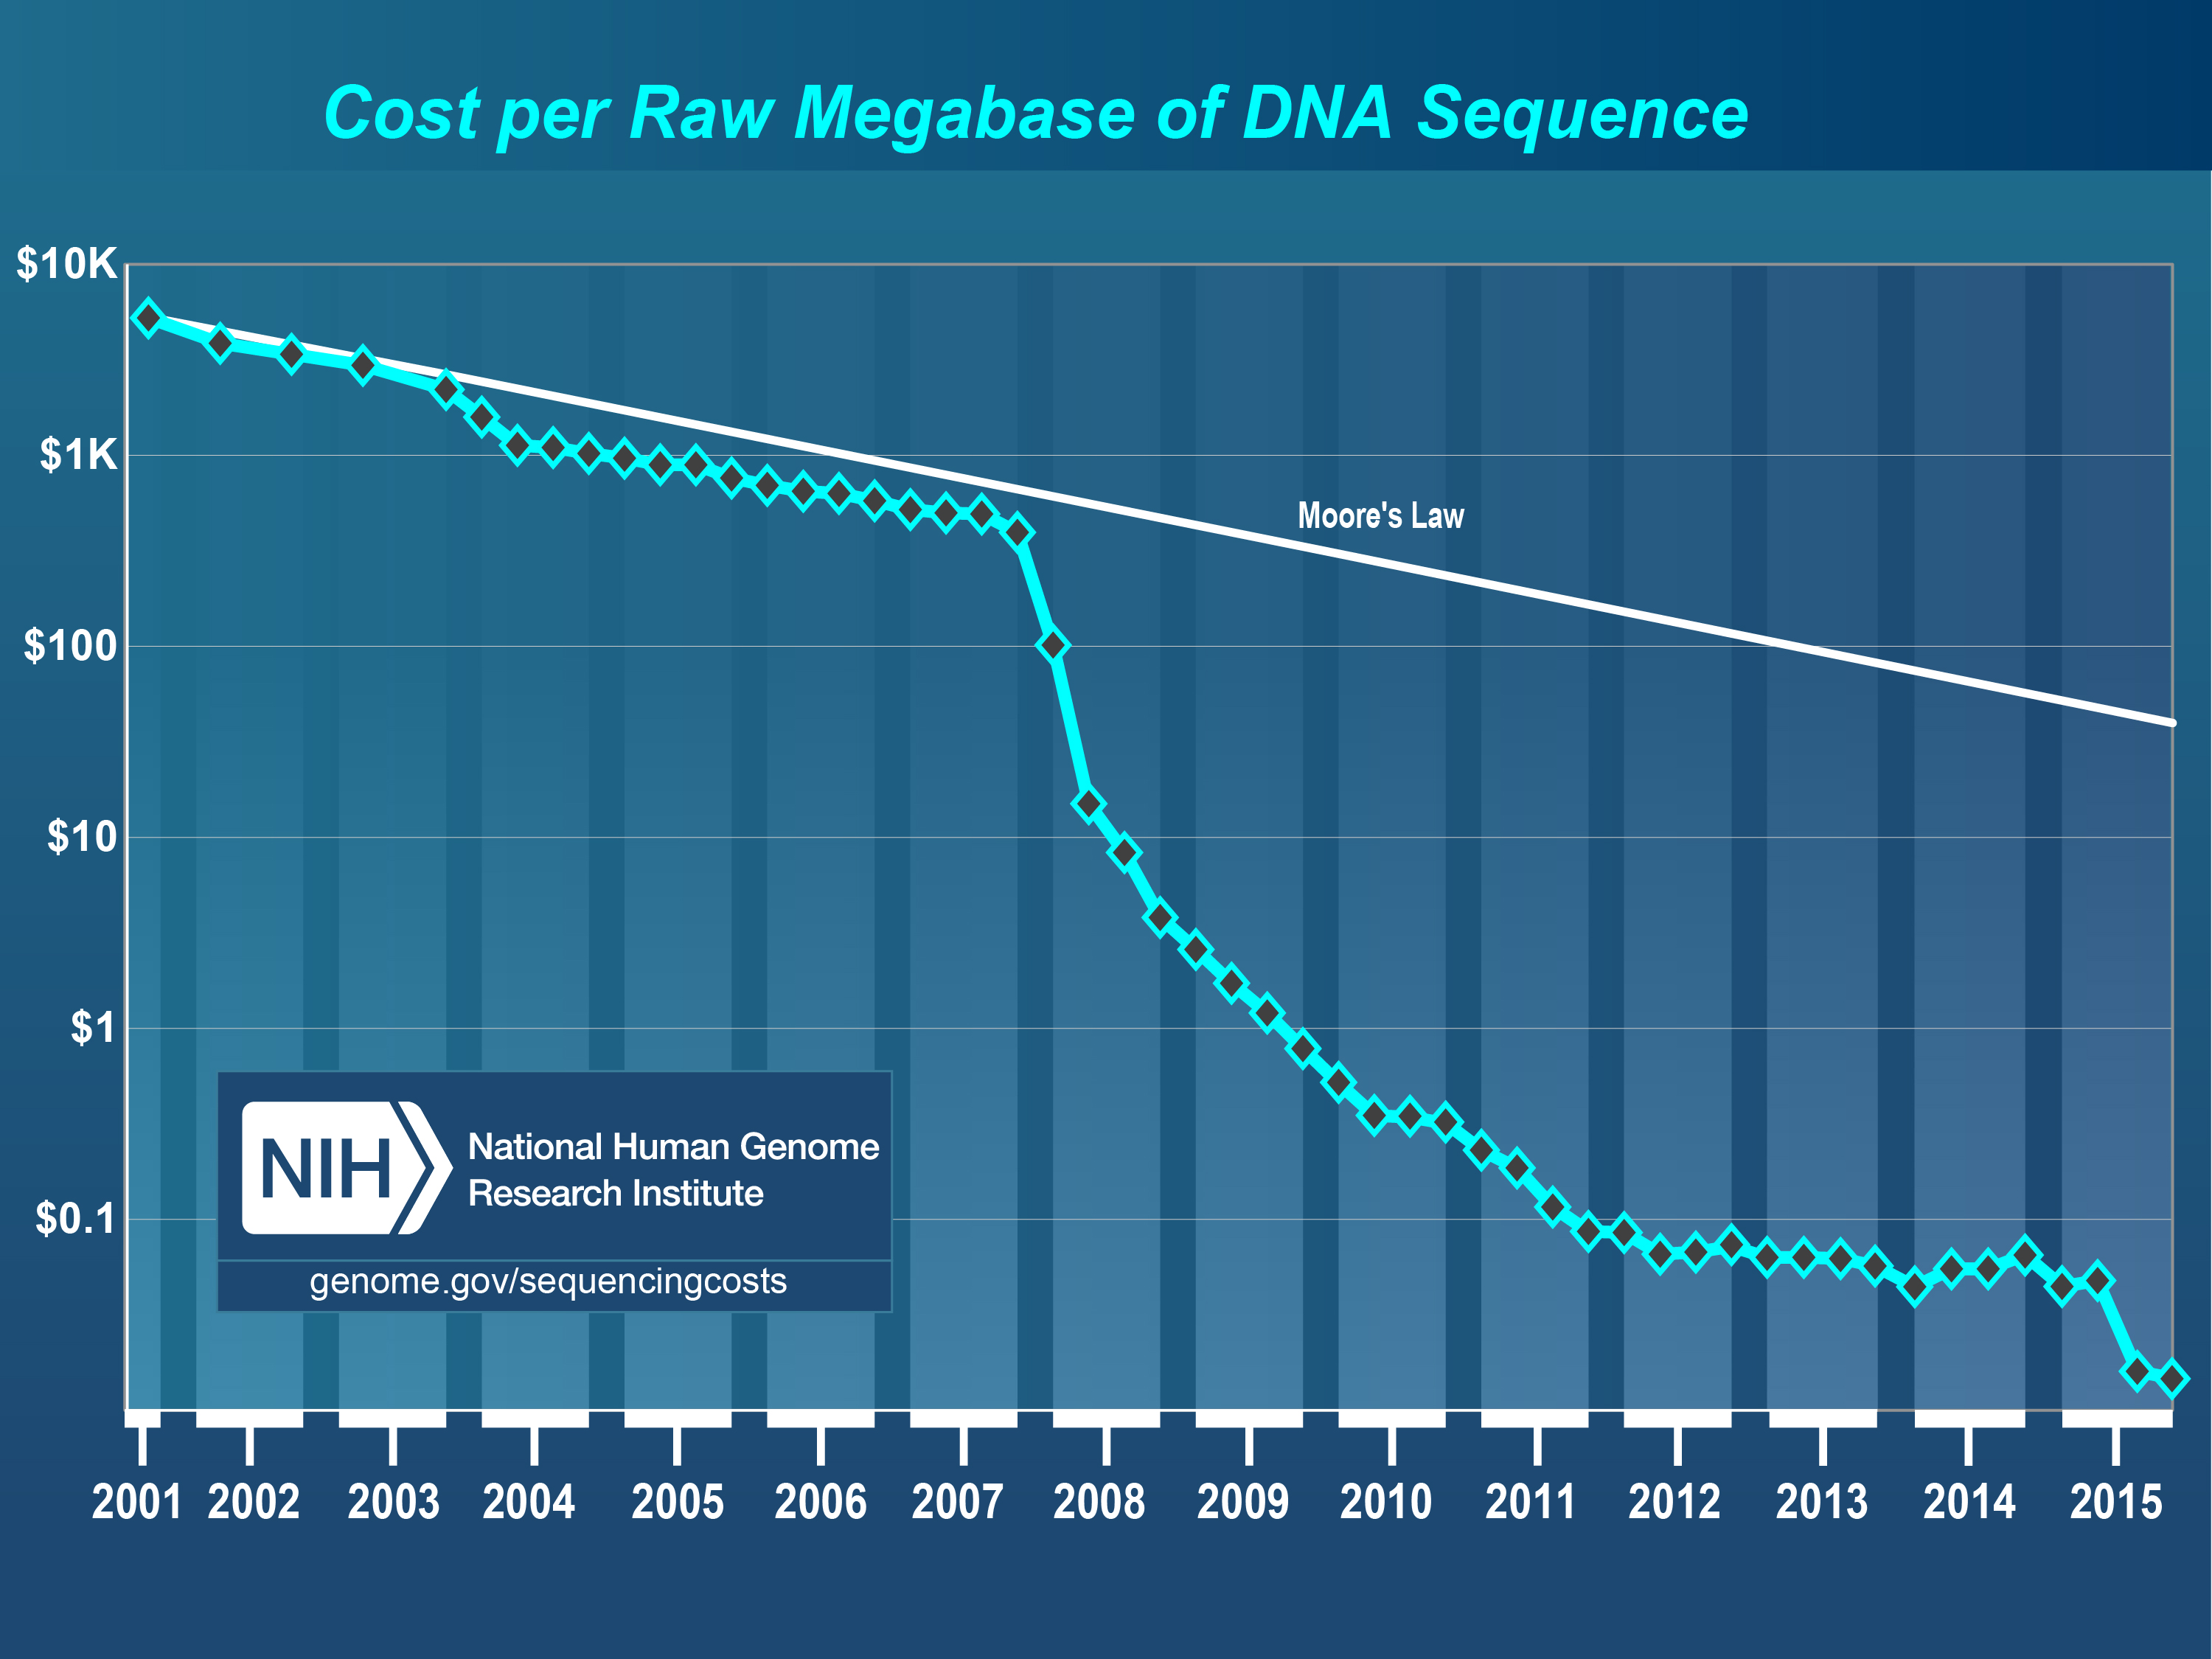
\includegraphics[scale=0.5]{costperMb2015_4.jpg}
\end{center}
\caption[Cost per raw megabase of DNA sequence from 2001 to 2015]{Cost per raw megabase of DNA sequence from 2001 to 2015. Straight line - Moore's Law, blue curve - cost in US dollars, Y-axis scale is logarithmic. Graph reproduced from \citep{wetterstrand2016}}
%Source:
\label{fig_dna_cost}
\end{figure}
Example of reference to a figure in the text (\Cref{fig_dna_cost}). Phasellus dolor neque, vehicula vestibulum semper at, facilisis eget libero. Mauris interdum magna molestie, auctor felis a, condimentum odio. Pellentesque habitant morbi tristique senectus et netus et malesuada fames ac turpis egestas. Suspendisse maximus lacinia dignissim. Maecenas pharetra accumsan metus, sagittis dictum purus sollicitudin eget. Curabitur ut porttitor arcu, ut porttitor ipsum. Vestibulum porttitor finibus sapien, ac pharetra odio bibendum nec. Nullam tincidunt dignissim risus imperdiet dictum.

Pellentesque habitant morbi tristique senectus et netus et malesuada fames ac turpis egestas. Suspendisse maximus lacinia dignissim. Maecenas pharetra accumsan metus, sagittis dictum purus sollicitudin eget. Curabitur ut porttitor arcu, ut porttitor ipsum. Vestibulum porttitor finibus sapien, ac pharetra odio bibendum nec. Nullam tincidunt dignissim risus imperdiet dictum.
\section{Example of a table}
Example of a table and here is the reference to \Cref{table_genomes}. Tables in, my opinion, are the hardest thing to make. Example how to reference several tables at once \Cref{table_genomes,table_vectors_108genomes,table_stats_108_network}. Notice there is NO SPACE between labels.

\begin{table}
\begin{center}
\begin{tabular}{|l|c|c|c|}
\hline
{\sc Organism}  &  {\sc Accession no.}  & {\sc Genome size} (bp)  & {\sc No. CDS} \\
\hline
{\it Mesorhizobium loti}          & NC\_002678 & 7036071 & 6743 \\
\hline
{\it Sinorhizobium meliloti}      & NC\_003047 & 3654135 & 3359 \\
\hline
{\it Bradyrhizobium japonicum}    & NC\_004463 & 9105828 & 8317 \\
\hline
{\it Rhodopseudomonas palustris}  & NC\_005296 & 5459213 & 4813 \\
\hline
{\it Bartonella quintana}         & NC\_005955 & 1581384 & 1142 \\
\hline
{\it Bartonella henselae}         & NC\_005956 & 1931047 & 1488 \\
\hline
{\it Rickettsia typhi}            & NC\_006142 & 1111496 & 837 \\
\hline
{\it Beijerinckia indica}         & NC\_010581 & 4170153 & 3569 \\
\hline
\end{tabular}
\end{center}
\caption{Whole-genome sequences used in this study}
\label{table_genomes}
\end{table}

\begin{table}[ht!]
\begin{center}
      \begin{tabular}{lcccc}
        \hline
\textbf{Genus} & \multicolumn{3}{c}{\textbf{Vectors}} & \textbf{Number of}\\ \cline{2-4}
{} & \textbf{Tick}  & \textbf{Louse}   & \textbf{Flea} &  \textbf{genomes}\\ 
\hline
\textit{Anaplasma} & 6 & 0 & 0 & \textbf{6} \\
\textit{Bartonella} & 0 & 2 & 4 & \textbf{6} \\
\textit{Borrelia} & 18 & 1 & 0 & \textbf{19}\\
\textit{Coxiella} & 5 & 0 & 0 & \textbf{5} \\
\textit{Ehrlichia} & 14 & 0 & 0 & \textbf{14} \\
\textit{Francisella} & 13 & 0 & 0 & \textbf{13}\\
\textit{Rickettsia} & 31 & 10 & 4 & \textbf{45}\\
\hline
\textbf{Total} & \textbf{87} & \textbf{13} & \textbf{8} & \textbf{108}\\
        \hline
      \end{tabular} 
\caption[Numbers of genomes examined and their vector association.]{Numbers of genomes examined and their vector association.}\label{table_vectors_108genomes}
\end{center}
\end{table}

\begin{table}[hb!]
\begin{center}
\begin{tabular}{lr}
\hline 
Number of organisms & 108 \\ 
Number of sequences & 127,409 \\ 
Number of edges & 1,970,450 \\ 
Number of clusters & 15,904 (100\%) \\ 
Number of singleton clusters & 6,372 (40\%) \\ 
Avg. vertex degree & 31 \\ 
\hline 
\end{tabular} 
\caption[Some statistics for the 108 genome network.]{Some statistics for the 108 genome network.}\label{table_stats_108_network}
\end{center}
\end{table}

Fusce ultricies pulvinar diam sed ultrices. Sed orci justo, rutrum in dolor a, consequat dictum mi. Sed luctus congue ex nec dignissim. Phasellus volutpat urna vestibulum ipsum vestibulum, quis venenatis justo consectetur. Nullam hendrerit nisl in rutrum convallis. Sed sit amet malesuada nisi. Phasellus dolor neque, vehicula vestibulum semper at, facilisis eget libero. Mauris interdum magna molestie, auctor felis a, condimentum odio. Pellentesque habitant morbi tristique senectus et netus et malesuada fames ac turpis egestas. Suspendisse maximus lacinia dignissim. Maecenas pharetra accumsan metus, sagittis dictum purus sollicitudin eget. Curabitur ut porttitor arcu, ut porttitor ipsum. Vestibulum porttitor finibus sapien, ac pharetra odio bibendum nec. Nullam tincidunt dignissim risus imperdiet dictum.

Pellentesque habitant morbi tristique senectus et netus et malesuada fames ac turpis egestas. Suspendisse maximus lacinia dignissim. Maecenas pharetra accumsan metus, sagittis dictum purus sollicitudin eget. Curabitur ut porttitor arcu, ut porttitor ipsum. Vestibulum porttitor finibus sapien, ac pharetra odio bibendum nec. Nullam tincidunt dignissim risus imperdiet dictum.
\section{Chapter section}
Fusce ultricies pulvinar diam sed ultrices. Sed orci justo, rutrum in dolor a, consequat dictum mi. Sed luctus congue ex nec dignissim. Phasellus volutpat urna vestibulum ipsum vestibulum, quis venenatis justo consectetur. Nullam hendrerit nisl in rutrum convallis. Sed sit amet malesuada nisi. Phasellus dolor neque, vehicula vestibulum semper at, facilisis eget libero. Mauris interdum magna molestie, auctor felis a, condimentum odio. Pellentesque habitant morbi tristique senectus et netus et malesuada fames ac turpis egestas. Suspendisse maximus lacinia dignissim. Maecenas pharetra accumsan metus, sagittis dictum purus sollicitudin eget. Curabitur ut porttitor arcu, ut porttitor ipsum. Vestibulum porttitor finibus sapien, ac pharetra odio bibendum nec. Nullam tincidunt dignissim risus imperdiet dictum.

Pellentesque habitant morbi tristique senectus et netus et malesuada fames ac turpis egestas. Suspendisse maximus lacinia dignissim. Maecenas pharetra accumsan metus, sagittis dictum purus sollicitudin eget. Curabitur ut porttitor arcu, ut porttitor ipsum. Vestibulum porttitor finibus sapien, ac pharetra odio bibendum nec. Nullam tincidunt dignissim risus imperdiet dictum.
\chapter{Chapter Five Title}
\section{Chapter section}
Fusce ultricies pulvinar diam sed ultrices. Sed orci justo, rutrum in dolor a, consequat dictum mi. Sed luctus congue ex nec dignissim. Phasellus volutpat urna vestibulum ipsum vestibulum, quis venenatis justo consectetur. Nullam hendrerit nisl in rutrum convallis. Sed sit amet malesuada nisi. Phasellus dolor neque, vehicula vestibulum semper at, facilisis eget libero. Mauris interdum magna molestie, auctor felis a, condimentum odio. Pellentesque habitant morbi tristique senectus et netus et malesuada fames ac turpis egestas. Suspendisse maximus lacinia dignissim. Maecenas pharetra accumsan metus, sagittis dictum purus sollicitudin eget. Curabitur ut porttitor arcu, ut porttitor ipsum. Vestibulum porttitor finibus sapien, ac pharetra odio bibendum nec. Nullam tincidunt dignissim risus imperdiet dictum.

Pellentesque habitant morbi tristique senectus et netus et malesuada fames ac turpis egestas. Suspendisse maximus lacinia dignissim. Maecenas pharetra accumsan metus, sagittis dictum purus sollicitudin eget. Curabitur ut porttitor arcu, ut porttitor ipsum. Vestibulum porttitor finibus sapien, ac pharetra odio bibendum nec. Nullam tincidunt dignissim risus imperdiet dictum.
\section{Chapter section}
Fusce ultricies pulvinar diam sed ultrices. Sed orci justo, rutrum in dolor a, consequat dictum mi. Sed luctus congue ex nec dignissim. Phasellus volutpat urna vestibulum ipsum vestibulum, quis venenatis justo consectetur. Nullam hendrerit nisl in rutrum convallis. Sed sit amet malesuada nisi. Phasellus dolor neque, vehicula vestibulum semper at, facilisis eget libero. Mauris interdum magna molestie, auctor felis a, condimentum odio. Pellentesque habitant morbi tristique senectus et netus et malesuada fames ac turpis egestas. Suspendisse maximus lacinia dignissim. Maecenas pharetra accumsan metus, sagittis dictum purus sollicitudin eget. Curabitur ut porttitor arcu, ut porttitor ipsum. Vestibulum porttitor finibus sapien, ac pharetra odio bibendum nec. Nullam tincidunt dignissim risus imperdiet dictum.

Pellentesque habitant morbi tristique senectus et netus et malesuada fames ac turpis egestas. Suspendisse maximus lacinia dignissim. Maecenas pharetra accumsan metus, sagittis dictum purus sollicitudin eget. Curabitur ut porttitor arcu, ut porttitor ipsum. Vestibulum porttitor finibus sapien, ac pharetra odio bibendum nec. Nullam tincidunt dignissim risus imperdiet dictum.

